\documentclass[10pt,aspectratio=43,mathserif,table]{beamer} 
%设置为 Beamer 文档类型,设置字体为 10pt,长宽比为16:9,数学字体为 serif 风格
\batchmode

\usepackage{graphicx}
\usepackage{animate}
\usepackage{hyperref}

%导入一些用到的宏包
\usepackage{amsmath,bm,amsfonts,amssymb,enumerate,epsfig,bbm,calc,color,ifthen,capt-of,multimedia,hyperref}
\usepackage{xeCJK} %导入中文包
\setCJKmainfont{SimHei} %字体采用黑体  Microsoft YaHei

\usetheme{Berlin} %主题
\usecolortheme{sustech} %主题颜色

\usepackage[ruled,linesnumbered]{algorithm2e}

\usepackage{fancybox}
\usepackage{xcolor}
\usepackage{times}
\usepackage{listings}

\usepackage{booktabs}
\usepackage{colortbl}

\newcommand{\Console}{Console}
\lstset{ %
	backgroundcolor=\color{white},   % choose the background color
	basicstyle=\footnotesize\rmfamily,     % size of fonts used for the code
	columns=fullflexible,
	breaklines=true,                 % automatic line breaking only at whitespace
	captionpos=b,                    % sets the caption-position to bottom
	tabsize=4,
	commentstyle=\color{mygreen},    % comment style
	escapeinside={\%*}{*)},          % if you want to add LaTeX within your code
	keywordstyle=\color{blue},       % keyword style
	stringstyle=\color{mymauve}\ttfamily,     % string literal style
	numbers=left, 
	%	frame=single,
	rulesepcolor=\color{red!20!green!20!blue!20},
	% identifierstyle=\color{red},
	language=c
}

\setsansfont{Microsoft YaHei}
\setmainfont{Microsoft YaHei}

\definecolor{mygreen}{rgb}{0,0.6,0}
\definecolor{mymauve}{rgb}{0.58,0,0.82}
\definecolor{mygray}{gray}{.9}
\definecolor{mypink}{rgb}{.99,.91,.95}
\definecolor{mycyan}{cmyk}{.3,0,0,0}

%题目,作者,学校,日期
\title{Reinventing the Wheel: Publishing High-quality Slides}
\subtitle{\fontsize{9pt}{14pt}\textbf{利用公共网关的SMS生态系统的安全性描述}}
\author{答辩人: 李易峰 \newline \newline 指导老师: 吴亦凡教授}
\institute{\fontsize{8pt}{14pt}中北大学英雄与联盟工程学院}
\date{\today}

%学校Logo
%\pgfdeclareimage[height=0.5cm]{sustech-logo}{sustech-logo.pdf}
%\logo{\pgfuseimage{sustech-logo}\hspace*{0.3cm}}

\AtBeginSection[]
{
	\begin{frame}<beamer>
	\frametitle{\textbf{目录}}
	\tableofcontents[currentsection]
\end{frame}
}
\beamerdefaultoverlayspecification{<+->}
% -----------------------------------------------------------------------------
\begin{document}
% -----------------------------------------------------------------------------

\frame{\titlepage}

\section[目录]{}   %目录
\begin{frame}{目录}
\tableofcontents
\end{frame}

% -----------------------------------------------------------------------------
\section{引言}  %引言
\subsection{研究背景}
\begin{frame}{研究背景}
\begin{columns}[T] % align columns
\begin{column}<0->{.40\textwidth}
	\begin{figure}[thpb]
		\centering
		\resizebox{1\linewidth}{!}{
			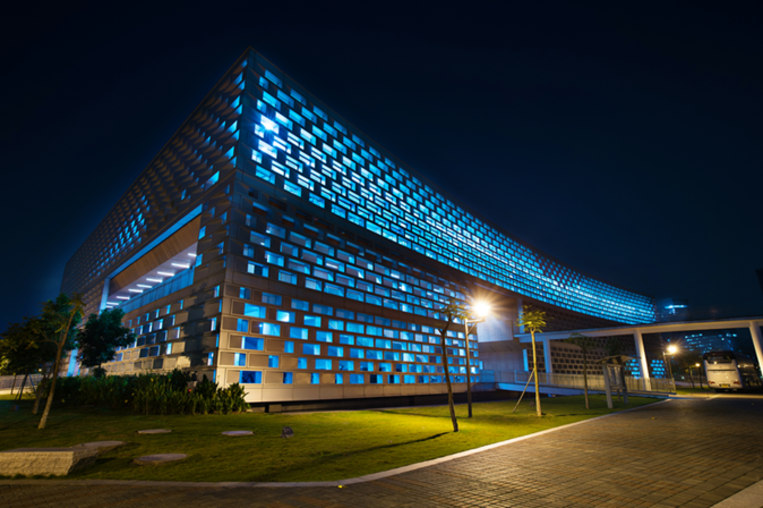
\includegraphics{figures/sustech.pdf}
		}
		%\includegraphics[scale=1.0]{figurefile}
		\caption{SUSTech Campus}
		\label{fig:campus}
	\end{figure}
\end{column}%
\hfill%
\begin{column}<0->{.65\textwidth}
	\begin{itemize}
		\item<1-> 短信息(SMS)成为现代通讯的重要组成部分
		\begin{itemize}
			\item<1-> 很多组织或网站使用短信息作为身份验证的辅助通道
		\end{itemize}
		\item<2-> 现代短消息的发送,在抵达终端之前不接触蜂窝网络
		\begin{itemize}
			\item<2-> 短信息(SMS)成为现代通讯的重要组成部分
		\end{itemize}
	\end{itemize}
\end{column}%
\end{columns}
\end{frame}
\subsection{主要工作}
\begin{frame}{主要工作}
完成这项工作需要如下步骤
\begin{block}{具体步骤}
\begin{itemize}
	\item<0->  对SMS数据进行迄今为止最大的挖掘分析
	\item<0->  评估良性短消息服务的安全态势
	\item<0->  刻画通过SMS网关进行的恶意行为
\end{itemize}
\end{block}
\end{frame}

 \begin{frame}
\frametitle{OTT服务}
\begin{figure}[!t]
	\centering
	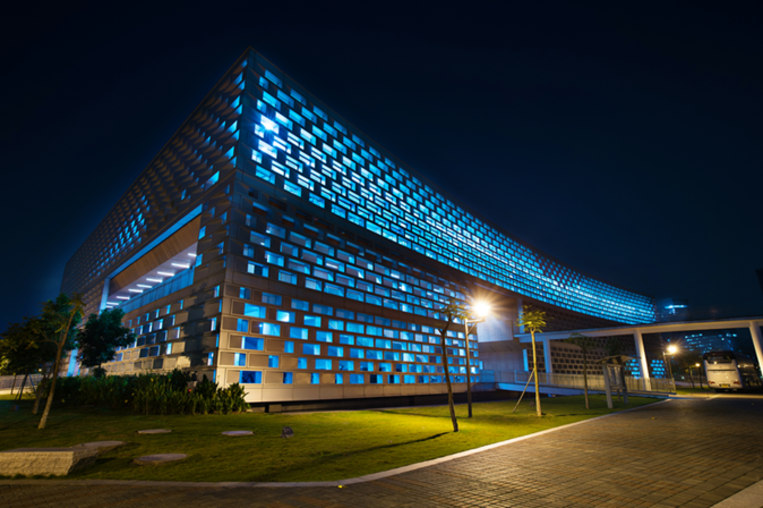
\includegraphics[width=2in]{figures/sustech.pdf}
	\caption{OTT服务}
	\label{figure3_OTT}
\end{figure}
\begin{center}
	OTT服务支持在数据网络上提供短信和语音等第三方服务。\\
	OTT可以使用云服务来存储和同步SMS到用户的其他设备。
\end{center}

\end{frame}



\section{词表示模型}  %自我介绍

\begin{frame}{词表示}
在NLP任务中,可以利用各种词表示模型,将“词”这种符号信息表示成数学上的向量形式。。将语义信息表示成稠密、低维的实值向量,这样就可以用计算向量之间相似度的方法(如余弦相似度),来计算语义的相似度。词的向量表示可以作为各种深度学习模型的输入来使用
\begin{block}{词表示模型分类}
	直接表示模型
	\begin{itemize}
		\item<0-> One-Hot Representation
	\end{itemize}
	
	分布式表示模型
	\begin{itemize}
		\item<0-> 计数模型(基于共现矩阵)
		\item<0-> 预测模型(基于神经网络)
	\end{itemize}
\end{block}
\end{frame}


\section{直接表示模型}
\begin{frame}{One-Hot Representation}
最简单直接的词表示是One-Hot Representation。考虑一个词表$ \mathbb V $,里面的每一个词$ w_i $都有一个编号$ i\in \{1,...,n\} $,那么词$ w_i $的one-hot表示就是一个维度为n的向量,其中第$ i $个元素值非零,其余元素全为0。例如:
\[  w_2=[0,1,0,...,0]^\top  \]
\[  w_3=[0,0,1,...,0]^\top  \]
\begin{block}{缺点}
	\begin{itemize}
		\item<0-> 彼此正交,不能反应词间的语义关系
		\item<0-> 稀疏表示,维度很高,和词典大小成正比
	\end{itemize}
\end{block}
\begin{center}
	\textcolor{mymauve}{仅仅是为了区分词,不包含语义信息,语义信息应该从上下文中挖掘}
\end{center}
\end{frame}


\section{研究方法与数据集特征}
\begin{frame}{研究方法与数据集特征}
\begin{columns}[c] % align columns
	\begin{column}<0->{.5\textwidth}
		\vspace*{1cm}
		\begin{itemize}
			\item 使用Scrapy框架爬取公共网关
		\end{itemize}
	
		\begin{itemize}
			\item 收集8个公共短信网关在14个月的数据
		\end{itemize}
	
		\begin{itemize}
			\item 共抓取386,327条数据
		\end{itemize}
    \end{column}%
\hfill%	
	\begin{column}<0->{.40\textwidth}
		\begin{table}
			\caption{公共网关抓取的信息数}
			\footnotesize
			\rowcolors{1}{mygray}{white}
			\begin{tabular}{|c|c|}
				\hline
				\textbf{Site}           & \textbf{Messages}\\
				\hline
				receivesmsonline.net    &81313\\
				\hline
				receive-sms-online.info &69389\\
				\hline
				receive-sms-now.com     &63797\\
				\hline
				hs3x.com               &55499\\
				\hline
				receivesmsonline.com    &44640\\
				\hline
				receivefreesms.com      &37485\\
				\hline
				receive-sms-online.com  &27094\\
				\hline
				e-receivesms.com       &7107\\
				\hline
			\end{tabular}
		\end{table}
    \end{column}%
\end{columns}
\end{frame}

\begin{frame}
\frametitle{消息聚类分析}
\begin{block}{\textbf{基本思路}}
	\begin{itemize}
		\item<0-> 使用编辑距离矩阵将类似的消息归于一张连通图中。
		\item<0-> 使用固定值替换感兴趣的消息,如代码、email地址。
		\item<0-> 查找归一化距离小于阈值的消息,并确定聚类边界。
	\end{itemize}
\end{block}

\begin{block}{\textbf{实现步骤}}
	\begin{enumerate}
		\item<0-> 加载所有消息。
		\item<0-> 用固定的字符串替换数字、电子邮件和URL以预处理消息。
		\item<0-> 将预处理后的信息按字母排序。
		\item<0-> 通过使用编辑距离阈值(0.9)来确定聚类边界。
		\item<0-> 手动标记各个聚类,以确定服务提供者、消息类别等。
	\end{enumerate}
\end{block}
\end{frame}

\section{算法和代码}
\subsection{算法}
\begin{frame}{算法}
\begin{algorithm}[H]
	\caption{HOSVD}
	\small 
	\KwIn{HOSVD($\mathcal{X},R_{1},R_{2}.....R_{N}$) }
	\KwOut{ $\mathcal{G},A_{(1)},A_{(2)}......A_{(N)} $ }
	
	\For{$k=1$ to $N$ }
	{
		$A_{(n)}\leftarrow R_{n}$left singular matrix of $X_{(n)}$
	}
	$\mathcal{G}=\leftarrow \mathcal{X} \times A_{(1)}^{T} \times A_{(2)}^{T}...... \times A_{(N)}^{T}$\\
	\Return $\mathcal{G},A_{(1)},A_{(2)}......A_{(N)} $
\end{algorithm}
\end{frame}

\subsection{代码}
\begin{frame}[fragile]{代码}
HOSVD在Python的代码实现和分析:
\lstinputlisting[lastline=11,
language=Python,
frame=single,
caption=First ten lines of some Python code,
label=python]
{HOSVD.py}
\end{frame}


\section{Future Work}
\begin{frame}{Future Work}  %将来可做的方向
\begin{itemize}
\item<0-> Get more people to try this
\item<0-> Benchmark the entire system in the wild
\item<0-> Profit!
\end{itemize}
\end{frame}

\begin{frame}{Thank you}
\begin{center}
\begin{minipage}{1\textwidth}
	\setbeamercolor{mybox}{fg=white, bg=black!50!blue}
 \begin{beamercolorbox}[wd=0.70\textwidth, rounded=true, shadow=true]{mybox}
\LARGE \centering Thank you for listening!  %结束语
\end{beamercolorbox}
 \end{minipage}
\end{center}
\end{frame}

\begin{frame}{Q\&A}
\begin{center}
	\begin{minipage}{1\textwidth}
		\setbeamercolor{mybox}{fg=white, bg=black!50!blue}
		\begin{beamercolorbox}[wd=0.70\textwidth, rounded=true, shadow=true]{mybox}
			\LARGE \centering  Questions?  %请求提问
		\end{beamercolorbox}
	\end{minipage}
\end{center}
\end{frame}

% -----------------------------------------------------------------------------
\end{document}
%文档结束